\documentclass{article}
\usepackage[paperwidth=7.16in,paperheight=6.70in,margin=0.06in]{geometry}
\usepackage{amsmath}
\usepackage{amssymb}
\usepackage{tikz}
\usetikzlibrary{arrows.meta,positioning,calc,backgrounds}
\pagestyle{empty}
\setlength{\parindent}{0pt}

% Restrained journal palette: gray for real features, blue for complex
% features, and violet for the dual-stream family/interactions.
\definecolor{realfill}{RGB}{246,246,246}
\definecolor{realedge}{RGB}{88,88,88}
\definecolor{complexfill}{RGB}{237,246,250}
\definecolor{complexedge}{RGB}{54,102,135}
\definecolor{dualfill}{RGB}{247,244,250}
\definecolor{dualedge}{RGB}{104,82,128}
\definecolor{attentionfill}{RGB}{250,247,239}
\definecolor{attentionedge}{RGB}{143,112,57}

\begin{document}
\centering
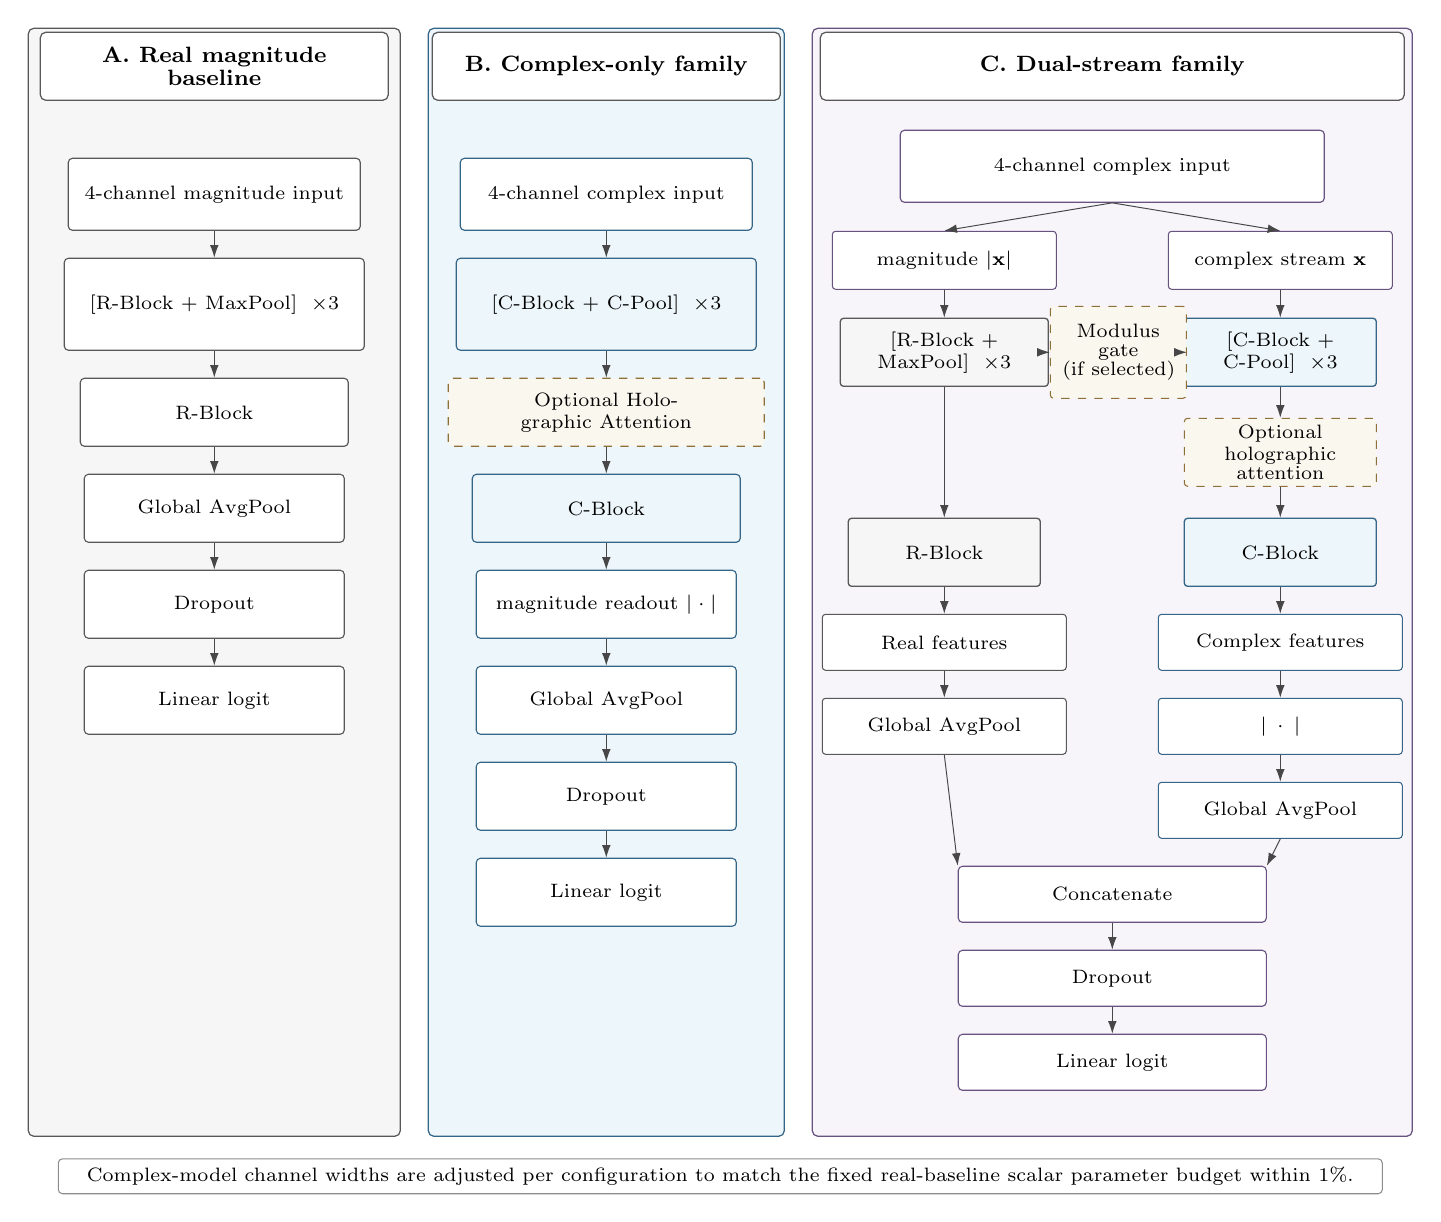
\begin{tikzpicture}[
  x=1in,y=1in,
  font=\scriptsize,
  >=Latex,
  arrow/.style={-{Latex[length=1.6mm,width=1.1mm]},line width=0.35pt,draw=black!72},
  lane/.style={rounded corners=2pt,line width=0.45pt,inner sep=0pt},
  header/.style={rounded corners=2pt,draw=black!65,fill=white,line width=0.45pt,
    minimum width=2.16in,minimum height=0.34in,align=center,text width=2.02in,
    font=\footnotesize\bfseries},
  narrowheader/.style={rounded corners=2pt,draw=black!65,fill=white,line width=0.45pt,
    minimum width=1.74in,minimum height=0.34in,align=center,text width=1.60in,
    font=\footnotesize\bfseries},
  narrowinput/.style={rounded corners=1.5pt,line width=0.42pt,minimum width=1.46in,
    minimum height=0.36in,align=center,text width=1.34in,inner sep=3pt},
  narrowblock/.style={rounded corners=1.5pt,line width=0.42pt,minimum width=1.34in,
    minimum height=0.34in,align=center,text width=1.24in,inner sep=2pt},
  narrowstage/.style={rounded corners=1.5pt,line width=0.42pt,minimum width=1.50in,
    minimum height=0.46in,align=center,text width=1.38in,inner sep=2pt},
  narrowoutput/.style={rounded corners=1.5pt,line width=0.40pt,minimum width=1.30in,
    minimum height=0.34in,align=center,text width=1.20in,inner sep=2pt},
  narrowinteraction/.style={rounded corners=1.5pt,draw=attentionedge,fill=attentionfill,dashed,line width=0.42pt,
    minimum width=1.58in,minimum height=0.34in,align=center,text width=1.46in,inner sep=2.5pt,
    font=\scriptsize},
  wideheader/.style={rounded corners=2pt,draw=black!65,fill=white,line width=0.45pt,
    minimum width=2.92in,minimum height=0.34in,align=center,text width=2.78in,
    font=\footnotesize\bfseries},
  wideinput/.style={rounded corners=1.5pt,line width=0.42pt,minimum width=2.12in,
    minimum height=0.36in,align=center,text width=1.98in,inner sep=3pt},
  repeatmark/.style={font=\scriptsize\bfseries,text=black!65,inner sep=0pt},
  input/.style={rounded corners=1.5pt,line width=0.42pt,minimum width=1.72in,
    minimum height=0.36in,align=center,text width=1.60in,inner sep=3pt},
  block/.style={rounded corners=1.5pt,line width=0.42pt,minimum width=1.58in,
    minimum height=0.34in,align=center,text width=1.48in,inner sep=2pt},
  stage/.style={rounded corners=1.5pt,line width=0.42pt,minimum width=1.76in,
    minimum height=0.46in,align=center,text width=1.64in,inner sep=2pt},
  output/.style={rounded corners=1.5pt,line width=0.40pt,minimum width=1.54in,
    minimum height=0.34in,align=center,text width=1.42in,inner sep=2pt},
  dualinput/.style={rounded corners=1.2pt,draw=dualedge,fill=white,line width=0.38pt,
    minimum width=1.12in,minimum height=0.29in,align=center,text width=1.02in,
    inner sep=1.5pt,font=\scriptsize},
  dualrepeatreal/.style={rounded corners=1.2pt,draw=realedge,fill=realfill,line width=0.38pt,
    minimum width=0.91in,minimum height=0.44in,align=center,text width=0.82in,
    inner sep=1.5pt,font=\scriptsize},
  dualrepeatcomplex/.style={rounded corners=1.2pt,draw=complexedge,fill=complexfill,line width=0.38pt,
    minimum width=0.91in,minimum height=0.44in,align=center,text width=0.82in,
    inner sep=1.5pt,font=\scriptsize},
  dualinteraction/.style={rounded corners=1.2pt,draw=attentionedge,fill=attentionfill,dashed,line width=0.38pt,
    minimum width=0.91in,minimum height=0.46in,align=center,text width=0.82in,
    inner sep=1.5pt,font=\scriptsize},
  dualbranch/.style={rounded corners=1.2pt,draw=dualedge,fill=white,line width=0.48pt,
    minimum width=0.96in,minimum height=0.34in,align=center,text width=0.84in,
    inner sep=1.5pt,font=\scriptsize},
  dualbranchreal/.style={dualbranch,draw=realedge,fill=realfill},
  dualbranchcomplex/.style={dualbranch,draw=complexedge,fill=complexfill},
  dualrepeatrealwide/.style={dualbranchreal,minimum width=1.04in,text width=0.92in},
  dualcallout/.style={rounded corners=1.2pt,draw=attentionedge,fill=attentionfill,dashed,line width=0.38pt,
    minimum width=0.68in,minimum height=0.46in,align=center,text width=0.56in,
    inner sep=1.5pt,font=\scriptsize},
  dualoptional/.style={rounded corners=1.2pt,draw=attentionedge,fill=attentionfill,dashed,line width=0.38pt,
    minimum width=0.96in,minimum height=0.34in,align=center,text width=0.84in,
    inner sep=1.5pt,font=\scriptsize},
  dualoutput/.style={rounded corners=1.2pt,draw=dualedge,fill=white,line width=0.38pt,
    minimum width=1.22in,minimum height=0.28in,align=center,text width=1.10in,
    inner sep=1.5pt,font=\scriptsize},
  dualfinal/.style={rounded corners=1.5pt,draw=dualedge,fill=white,line width=0.40pt,
    minimum width=1.54in,minimum height=0.28in,align=center,text width=1.42in,
    inner sep=2pt,font=\scriptsize},
  dualstage/.style={rounded corners=1.5pt,draw=dualedge,fill=white,line width=0.42pt,
    minimum width=1.98in,minimum height=0.56in,align=center,text width=1.84in,
    inner sep=2pt,font=\scriptsize},
  interaction/.style={rounded corners=1.5pt,draw=attentionedge,fill=attentionfill,dashed,line width=0.42pt,
    minimum width=1.98in,minimum height=0.34in,align=center,text width=1.84in,inner sep=2.5pt,
    font=\scriptsize},
  note/.style={rounded corners=1.5pt,draw=black!45,fill=white,line width=0.38pt,
    minimum width=6.62in,align=center,text width=6.40in,inner sep=3pt,font=\scriptsize}
]

% Three aligned family panels.
\begin{scope}[on background layer]
  \path[lane,draw=realedge,fill=realfill] (-3.46,3.12) rectangle (-1.60,-2.42);
  \path[lane,draw=complexedge,fill=complexfill] (-1.46,3.12) rectangle (0.32,-2.42);
  \path[lane,draw=dualedge,fill=dualfill] (0.46,3.12) rectangle (3.46,-2.42);
\end{scope}

% -------------------------------------------------------------------------
% A. Real magnitude baseline
% -------------------------------------------------------------------------
\node[narrowheader] (realhead) at (-2.53,2.93) {A. Real magnitude\\[-1pt] baseline};
\node[narrowinput,draw=realedge,fill=white] (rinput) at (-2.53,2.29) {4-channel magnitude input};
\node[narrowstage,draw=realedge,fill=white] (rrepeat) at (-2.53,1.74)
  {[R-Block + MaxPool]\; $\times 3$};
\node[narrowblock,draw=realedge,fill=white] (rblock4) at (-2.53,1.20) {R-Block};
\node[narrowoutput,draw=realedge,fill=white] (rgap) at (-2.53,0.72) {Global AvgPool};
\node[narrowoutput,draw=realedge,fill=white] (rdrop) at (-2.53,0.24) {Dropout};
\node[narrowoutput,draw=realedge,fill=white] (rlogit) at (-2.53,-0.24) {Linear logit};
\foreach \a/\b in {rinput/rrepeat,rrepeat/rblock4,rblock4/rgap,rgap/rdrop,rdrop/rlogit}
  {\draw[arrow] (\a.south) -- (\b.north);}

% -------------------------------------------------------------------------
% B. Complex-only family
% -------------------------------------------------------------------------
\node[narrowheader] (chead) at (-0.57,2.93) {B. Complex-only family};
\node[narrowinput,draw=complexedge,fill=white] (cinput) at (-0.57,2.29) {4-channel complex input};
\node[narrowstage,draw=complexedge,fill=complexfill] (crepeat) at (-0.57,1.74)
  {[C-Block + C-Pool]\; $\times 3$};
\node[narrowinteraction] (cinteraction) at (-0.57,1.20) {Optional Holographic Attention};
\node[narrowblock,draw=complexedge,fill=complexfill] (cblock4) at (-0.57,0.72) {C-Block};
\node[narrowoutput,draw=complexedge,fill=white] (cmag) at (-0.57,0.24)
  {magnitude readout $|\cdot|$};
\node[narrowoutput,draw=complexedge,fill=white] (cglobal) at (-0.57,-0.24)
  {Global AvgPool};
\node[narrowoutput,draw=complexedge,fill=white] (cdrop) at (-0.57,-0.72) {Dropout};
\node[narrowoutput,draw=complexedge,fill=white] (cclass) at (-0.57,-1.20) {Linear logit};
\foreach \a/\b in {cinput/crepeat,crepeat/cinteraction,cinteraction/cblock4,cblock4/cmag,cmag/cglobal,cglobal/cdrop,cdrop/cclass}
  {\draw[arrow] (\a.south) -- (\b.north);}

% -------------------------------------------------------------------------
% C. Dual-stream family
% -------------------------------------------------------------------------
\node[wideheader] (dhead) at (1.96,2.93) {C. Dual-stream family};
\node[wideinput,draw=dualedge,fill=white] (dinput) at (1.96,2.43) {4-channel complex input};
\node[dualinput] (drealin) at (1.12,1.96) {magnitude $|\mathbf{x}|$};
\node[dualinput] (dcomplexin) at (2.80,1.96) {complex stream $\mathbf{x}$};
\draw[arrow] (dinput.south) -- (drealin.north);
\draw[arrow] (dinput.south) -- (dcomplexin.north);
\node[dualrepeatrealwide] (drepeatreal) at (1.12,1.50) {[R-Block + MaxPool]\; $\times 3$};
\node[dualbranchcomplex] (drepeatcomplex) at (2.80,1.50) {[C-Block + C-Pool]\; $\times 3$};
\draw[arrow] (drealin.south) -- (drepeatreal.north);
\draw[arrow] (dcomplexin.south) -- (drepeatcomplex.north);
\node[dualcallout] (dgate) at (1.99,1.50) {Modulus\\[-1pt]gate\\[-1pt]\mbox{(if selected)}};
\draw[arrow] (drepeatreal.east) -- (dgate.west);
\draw[arrow] (drepeatcomplex.west) -- (dgate.east);
\node[dualoptional] (dcomplexinteraction) at (2.80,1.00) {Optional holographic\\[-1pt] attention};
\node[dualbranchreal] (dblock4real) at (1.12,0.50) {R-Block};
\node[dualbranchcomplex] (dblock4complex) at (2.80,0.50) {C-Block};
\draw[arrow] (drepeatreal.south) -- (dblock4real.north);
\draw[arrow] (drepeatcomplex.south) -- (dcomplexinteraction.north);
\draw[arrow] (dcomplexinteraction.south) -- (dblock4complex.north);
\node[dualoutput,draw=realedge] (drealfeatures) at (1.12,0.05) {Real features};
\node[dualoutput,draw=realedge] (drealgap) at (1.12,-0.37) {Global AvgPool};
\node[dualoutput,draw=complexedge] (dcomplexfeatures) at (2.80,0.05) {Complex features};
\node[dualoutput,draw=complexedge] (dcmag) at (2.80,-0.37) {$|\cdot|$};
\node[dualoutput,draw=complexedge] (dcglobal) at (2.80,-0.79) {Global AvgPool};
\draw[arrow] (dblock4real.south) -- (drealfeatures.north);
\draw[arrow] (drealfeatures.south) -- (drealgap.north);
\draw[arrow] (dblock4complex.south) -- (dcomplexfeatures.north);
\draw[arrow] (dcomplexfeatures.south) -- (dcmag.north);
\draw[arrow] (dcmag.south) -- (dcglobal.north);
\node[dualfinal] (dconcat) at (1.96,-1.21) {Concatenate};
\node[dualfinal] (ddrop) at (1.96,-1.63) {Dropout};
\node[dualfinal] (dlogit) at (1.96,-2.05) {Linear logit};
\draw[arrow] (drealgap.south) -- (dconcat.north west);
\draw[arrow] (dcglobal.south) -- (dconcat.north east);
\draw[arrow] (dconcat.south) -- (ddrop.north);
\draw[arrow] (ddrop.south) -- (dlogit.north);

% Single parameter-matching note.
\node[note] at (0,-2.62)
  {Complex-model channel widths are adjusted per configuration to match the fixed real-baseline scalar parameter budget within 1\%.};

\end{tikzpicture}

\vspace{0.07in}
\begin{minipage}{6.94in}
\scriptsize
\textbf{Figure 3.} High-level model families evaluated in the study. The real baseline processes coil magnitudes, the complex-only family retains complex-valued features until magnitude readout, and the dual-stream family processes magnitude and complex representations in parallel before feature fusion. Repeated processing stages are shown using $\times 3$ notation.
\end{minipage}
\end{document}
